%This is part of Un soupçon de mathématique sans être agressif pour autant
% Copyright (c) 2012-2013
%   Laurent Claessens, Pauline Klein
% See the file fdl-1.3.txt for copying conditions.

%+++++++++++++++++++++++++++++++++++++++++++++++++++++++++++++++++++++++++++++++++++++++++++++++++++++++++++++++++++++++++++
\section{Courbe représentative d'une fonction}
%+++++++++++++++++++++++++++++++++++++++++++++++++++++++++++++++++++++++++++++++++++++++++++++++++++++++++++++++++++++++++++

% AFAIRE : un beau graphique sympa à projeter sur lequel on peut parler de croissance d'image et d'antécédents.

%TODO : il faut essayer de refaire une figure pour tous les dessins de Pauline.
Soit $f$ une fonction définie sur un ensemble $\defD$.

\begin{definition}
    On appelle \defe{représentation graphique}{représentation graphique (d'une fonction)}, ou le \defe{graphe}{graphe} de $f$, l'ensemble des points $(x,y)$ tels que $x\in\defD$ et $y=f(x)$.

    Lorsque \( y=f(x)\), le nombre \( y\) est l'\defe{image}{image par une fonction} de \( x\) par la fonction \( f\) et \( x\) est \emph{un} \defe{antécédent}{antécédent} de \( y\).
\end{definition}

\begin{Aprojeter}

    \begin{Aretenir}
        La règle d'or des graphiques : le point de coordonnées \( (a;b)\) est sur le graphique de la fonction \( f\) si et seulement si \( f(a)=b\).
    \end{Aretenir}

    %The result is on figure \ref{LabelFigAHAbqhj}. % From file AHAbqhj
    %\newcommand{\CaptionFigAHAbqhj}{<+Type your caption here+>}
    %\input{Fig_AHAbqhj.pstricks}

    %\begin{wrapfigure}{r}{7.0cm}
    %   \vspace{-0.5cm}        % à adapter.
    %   \centering
    %\end{wrapfigure}

    \begin{multicols}{2}

    À propos du graphe ci-contre :
    \begin{enumerate}
        \item
            Quel est l'ensemble de définition de la fonction \( f\) ?
        \item
            Quelle est l'image de \( 1\) par \( f\) ?
        \item
            Donner un antécédent de \( 3\).
        \item
            Quels sont les antécédents de \( -1\) ?
    \end{enumerate}
        
        \columnbreak

    \begin{center}
       \input{Fig_AHAbqhj.pstricks}
    \end{center}

    \end{multicols}
\end{Aprojeter}

%Quelque conseils pour dessiner.
%\begin{itemize}
%    \item
%        Pour une valeur $x$ sur l'axe des abscisses, il y a un et un seul point d'abscisse $x$ sur la courbe.
%    \item
%        Pour tracer une courbe, il faut placer des points. Plus on choisit de points, plus la courbe sera précise.
%    \item
%        Si possible, trouver quelque valeurs clefs. Par exemple on cherchera les points d'intersection entre les axes et les courbe. Le point \( (0,f(0)) \) est intéressant à mettre, ainsi que les points \( x\) tels que \( f(x)=0\).
%\end{itemize}


%\newcommand{\CaptionFigExFonction}{Comment tracer la fonction \( f\colon x\to 2x+1\) ?}
%\input{Fig_ExFonction.pstricks}

%Nous donnons à la figure \ref{LabelFigExFonction} le tracé de la fonction \( f(x)=2x+1\). La figure \ref{LabelFigExFonctionssLabelSubFigExFonction0} donne quelque points du graphe de la fonction. La figure \ref{LabelFigExFonctionssLabelSubFigExFonction1} donne le graphe complet de la fonction. Comment le construit-on ? Par définition pour chaque \( x\) sur l'axe des abscisses (il y en a une infinité), il faut calculer le nombre \( f(x)\) et mettre dans le plan le point de coordonnées \( \big( x,f(x) \big)\).

%En pratique, il n'est pas possible de calculer \( f(x)\) pour \emph{tous} les \( x\) réels\footnote{Chuck Norris peut le faire.}. C'est pourquoi nous nous contentons qu'en calculer quelque uns, et nous les relions «le plus intelligemment possible».


%---------------------------------------------------------------------------------------------------------------------------
\subsection{Ce qui n'est pas une fonction}
%---------------------------------------------------------------------------------------------------------------------------

%    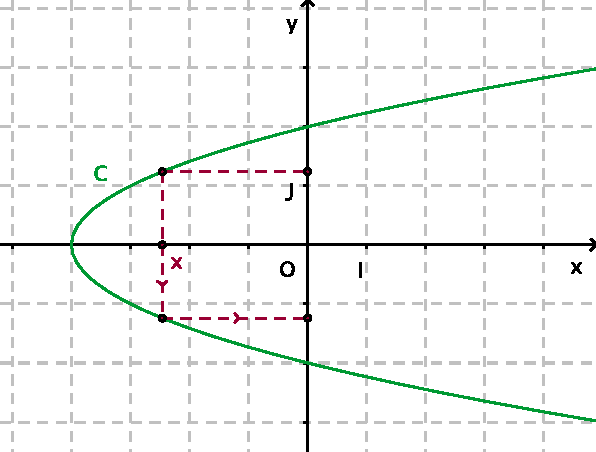
\includegraphics[width=5cm]{F_NonFct.pdf}

\begin{multicols}{2}
    Cette courbe ne représente pas une fonction, car à partir de \( x=-4\), les nombres ont deux images. Les courbes données par des fonctions sont des courbes acceptant une seule ordonnée pour chaque abscisse.

\columnbreak

%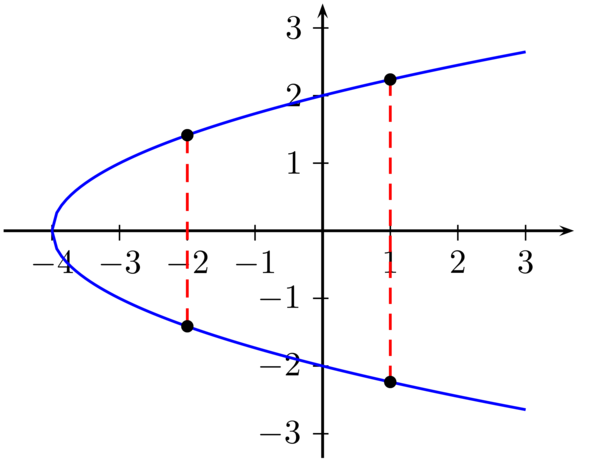
\includegraphics{Picture_FIGLabelFigPasFonctionYoQfSuPICTPasFonctionYoQfSu-for_eps.pdf}

\input{Fig_PasFonctionYoQfSu.pstricks}

\end{multicols}
